\section{Vorlesung 09.12.2016 (Spezialvorlesung 1)}
\subsection{Phylogenetische Kombinatorik}
		
\begin{itemize}
	\item Distanz Methoden / Clustering $\leftrightarrow$ Netzwerke statt Bäume 
	\item Supertree / Tripel-Methoden
\end{itemize}
\subsubsection{Phylogenetische Distanzen}

x = \color{red}0 \color{green}1 \color{red}1 \color{green}1 \color{red}0 \color{green}0 1\\\color{black}
y = \color{red}1 \color{green}1 \color{red}0 \color{green}1 \color{red}1 \color{green}0 1\\
\color{black}$\rightarrow$ Hamming Distanz: $d_h(x,y) = 3$

\begin{center}
	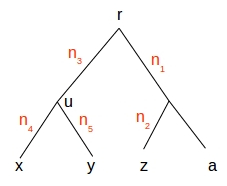
\includegraphics[scale=0.9]{lectures/161209/pix/pic1.jpg}
\end{center}

Evolutionäre Distanz = Evol. Ereignisse; die x,y trennen	
\begin{align*}
	d_E (z,x) &= n_2 + n_1 + n_3 + n_4\\
	d_E (x,y) &= n_4 + n_5\\
	d_E (z,y) &= n_2 + n_1 + n_3 + n_5
\end{align*}
\begin{align*}
	d_E (z,x) &= d_E (z,u) + n_4\\
	d_E (z,y) &= d_E (z,u) + n_5\\
	d_E (z,x) + d_E (z,y) &= 2 d_E(z,u) + n_4 + n_5
\end{align*}
\begin{align*}
	d_E (z,u) &= \frac{1}{2} \lbrace d_E (z,x) + d_E (z,y) - d_E (x,y) \rbrace
\end{align*}

\begin{itemize}
	\item messbare Daten: Abstände zwischen Taxa $\equiv$ Blätter des Baumes
	\item Position der Wurzel:
		\begin{itemize}
			\item[*] jede messbare Distanz enthält entweder $(n_1 + n_3)$ oder weder $n_1$ noch $n_3$
			\item[*] genaue Position der Wurzel NICHT bestimmbar
			\item[$\rightarrow$] ungewurzelte Bäume
		\end{itemize}
\end{itemize}

\begin{center}
	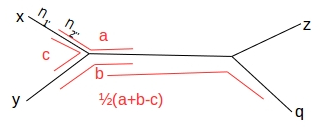
\includegraphics[scale=1]{lectures/161209/pix/pic2.jpg}		
\end{center}

Entspricht Hamming-Distanz der evolutionären Distanz: $d_H (x,y) \Leftrightarrow d_E (x,y)$?
Nein wegen möglichen Rückmutationen, daher: $\underbrace{d_H (x,y)}_{messbar} \leq \underbrace{d_E (x,y)}_{\text{nicht messbar}}$

\begin{center}
	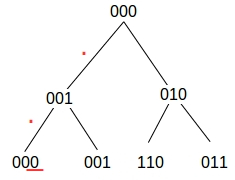
\includegraphics[scale=1]{lectures/161209/pix/pic3.jpg}
\end{center}

\newpage	

\subsubsection{Modell für Sequenzevolution}
\textbf{Markov:}
\begin{align*}
	P_{a,b}(\tau) &:= P(a | b, \tau) = \biggl[e^{\mu \tau R} \biggr]_{a,b}
\end{align*}
$P(a | b, \tau)$: die Wahrscheinlichkeit a zu sehen wen ich b gesehen habe nach einer Zeit $\tau$
\\\\
$\mu = $ Mutationsrate\\
$\tau = $ Zeit\\
$R = $ Matrix Mutationsmodell

\begin{align*}
	R_1 = \begin{pmatrix}
		-1 & 1\\
		 1 &-1
	\end{pmatrix}
\end{align*}
\begin{align*}
	R_2 = \begin{pmatrix}
		-3 & 1 & 1 & 1\\
		 1 &-3 & 1 & 1\\
		 1 & 1 &-3 & 1\\
		 1 & 1 & 1 &-3
	\end{pmatrix}
\end{align*}
\begin{align*}
	Taylorreihe: e^{\mu * \tau * R} &:= I + \tau * \mu * R + \frac{1}{2!} * \tau^2 * \mu^2 * R^2 + \frac{1}{3!} * \tau^3 * \mu^3 * R^3 + ...
\end{align*}
mit $I$=Einheitsmatrix
\begin{align*}
	P_{a,b}(\tau) &= \delta_{a,b} + \tau * \mu * R_{a,b} + ...
\end{align*}

mit Kronecker-Delta: $\delta_{a,b}
\begin{cases}
	0 \text{ wenn } a\neq b\\
	1 \text{ wenn } a = b\\
\end{cases}
$
\\
\underline{mit $R_1$-Matrix:}\\
\textbf{a = b:} $P_{a,a}(\tau) = 1 + \tau * \mu * (-1) + \sigma (\tau ^2) = 1 - \tau * \mu + \sigma (\tau ^2)$\\
\textbf{a $\neq$ b:} $P_{a,b}(\tau) = 0 + \tau * \mu * 1 + \sigma (\tau ^2) = \tau * \mu + \sigma (\tau ^2)$
\\\\
$\sigma (\tau ^2) = $ Rückmutation, $\tau, \mu$ können nicht getrennt werden $\rightarrow$ Anzahl Ereignisse
 
\begin{center}
	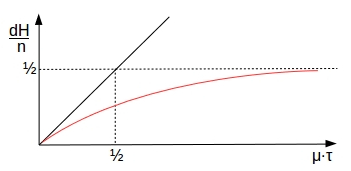
\includegraphics[scale=1.2]{lectures/161209/pix/pic4.jpg}
\end{center}

\begin{align*}
	\frac{dH}{n}~=~P_{a,b} (\tau) | \{a \neq b\}~=~\tau * \mu + \sigma (\tau ^2)
\end{align*}
\begin{align*}
	\lim\limits_{\tau \rightarrow \infty} P_{a,b} (\tau)~=~ \frac{1}{2}
\end{align*}
\begin{align*}
 	\frac{dH}{n}~=~ \frac{1}{2} (1 - e^{-\tau * \mu})
\end{align*} 
$\frac{1}{2} =$ \color{orange} weil 2 Buchstaben\color{black}\\
$\tau * \mu =$ \color{orange} $dE$ \color{black}

\begin{align*}
 	dH(\tau) ~&=~ \sum \limits_{b \in A} \sum \limits_{a \neq b}  f_b^{Anfang} * P_{a,b}(\tau)\\
 	2 \frac{dH}{n} ~&=~ 1 - e^{-\tau * \mu}\\
 	e^{-\tau * \mu} ~&=~ 1 - 2 \frac{dH}{n}\\
 	\tau * \mu ~&=~ -ln (1 - 2 \frac{dH}{n}) = dE
\end{align*} 
\\Gilt nur für einfachen binären Fall (siehe $R_1$)
\subsubsection{Evolutionäre Distanzen $\rightarrow$ Baum}
geg.: Baum T, Kantenlängen l: E(T) $\rightarrow \mathbb {R}_0^+$\\

\hspace{2cm} $\Rightarrow$ Distanzen $d(x,y) = \sum \limits_{e \in Pfad_T (x,y)} l(e)$ \color{orange}(*)\color{black}\\

\textbf{Definition:}\\
Eine metrische Distanz $d: X \times X \rightarrow \mathbb {R}_0^+$ \\
heißt ADDITIV, wenn es einen Baum T\\
mit Blättern X und Kantenlängen l gibt sodass \color{orange}(*)\color{black} stimmt	

Distanz heißt metrisch wenn:
\begin{itemize}
	\item[(i)] $d(x,x) = 0$
	\item[(ii)] $d(x,y) = 0 \rightarrow x = y$
	\item[(iii)] $d(x,y) = d(y,x)$
	\item[(iv)] $d(x,y) + d(y,z) \geq d(x,z)\ \forall\ x, y, z \in X$ (Dreiecksungleichung)
\end{itemize}

\newpage
\underline{Wann ist eine Distanz additiv?}

Bem.: wenn $l(e) > 0$ für alle Kanten e $\Rightarrow$ additive Distanz ist metrisch

\begin{center}
	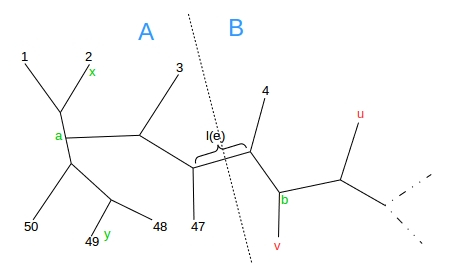
\includegraphics[scale=1]{lectures/161209/pix/pic5.jpg}
\end{center}

Kante e induziert eine Partition von T und damit X in genau 2 Teilmengen (A,B), nicht leer $\Rightarrow$ \textcolor{purple}{SPLIT}

\begin{align*}
 	&A \cap B = \emptyset \\
 	&A \neq 0 \\
 	&B \neq 0 \\
 	&A \cup B = X
\end{align*}

\underline{Was zeichnet Splits, die einer Kante im Baum entsprechen, aus?}\\\\
Sei A $|$ B der Split, der zu e gehört\\
$x,y \in A$, $u,v \in B$, a innerer Knoten in A, b innerer Knoten in B:\\
l(e) = $\min \limits_{a,b} d(a,b)$ für a,b als Knoten für Kante e gewählt


\begin{center}
	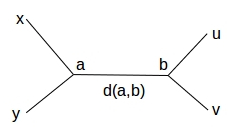
\includegraphics[scale=1]{lectures/161209/pix/pic6.jpg}\\
	$\underbrace{d(x,u) + d(y,v)}_{=Q} - d(x,y) - d(u,v) = 2d(a,b)$
\end{center}

\newpage

Da es ein Baum ist auch alternativ:
$\underbrace{d(x,\underline{v}) + d(y,\underline{u})}_{=Q} - d(x,y) - d(u,v) = 2d(a,b)$\\
$\rightarrow$ Q muss in Baum das Gleiche sein.\\\\
$\Rightarrow$ $l(e) = \frac{1}{2} \min \limits_{\substack{x,y \in A\\ u,v \in B}} d(x,u) + d(y,v) - d(x,y) - d(u,v)$\\\\
oder $l(e) = \frac{1}{2} \min \limits_{\substack{x,y \in A\\ u,v \in B}} d(x,\underline{v}) + d(y,\underline{u}) - d(x,y) - d(u,v)$
\\\\
\underline{Was wenn A, B nicht zu einer Kante gehören?}
\begin{center}
	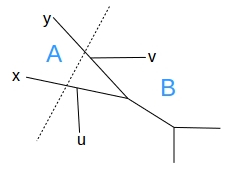
\includegraphics[scale=1]{lectures/161209/pix/pic7.jpg}
\end{center}
$\Rightarrow$ l(e) $<$ 0 da:
\begin{center}
	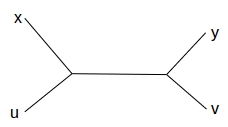
\includegraphics[scale=1]{lectures/161209/pix/pic8.jpg}\\
	$\Rightarrow$ $\underbrace{d(x,u) + d(y,v)}_{<d(x,y) + d(u,v)} - \underbrace{(d(x,y) + d(u,v))}_{>d(x,u) + d(y,v)}$
\end{center}

wenn A $|$ B kein Split von T $\Rightarrow l(A|B) < 0$\\
wenn A $|$ B Split von T $\Rightarrow l(A|B) = l(e)$ 
\\\\
\fcolorbox{red}{white}{\parbox{\linewidth}{
$l(A|B) = \frac{1}{2} \min \limits_{\substack{x,y \in A\\ u,v \in B}} d(x,u) + d(y,v) - d(x,y) - d(u,v)$}}
\\\\
für je 4 Blätter betrachte:\\
\begin{align*}
 	d(x,u) + d(y,v) - d(x,y) - d(u,v)\\
 	d(x,v) + d(y,u) - d(x,y) - d(u,v)\\
 	d(x,y) + d(u,v) - d(x,u) - d(y,v)
\end{align*}
2 dieser 3 Terme sind gleich, die 3te ist nicht größer. (da auch 0 zulässig)\\
$\Rightarrow$ wenn das für alle (x,y),(u,v) gilt, dann ist Metrik aus Baum abgeleitet

\newpage
\subsubsection{Splitsystem eines Baums}

$\sum (T) = \{$ splits in T, also die, die zu Kanten gehören.$\}$

\begin{enumerate}
	\item[1)] $ \{ x \}~|~X \setminus \{ x \} \in \sum (T)$ für alle $x \in X$ $\rightarrow$ triviale Splits
\end{enumerate}

\underline{zwei verschiedene Splitvarianten:}
\begin{center}
	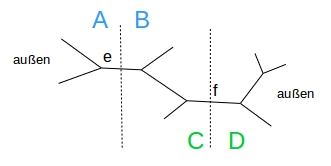
\includegraphics[scale=1.25]{lectures/161209/pix/pic9.jpg}
\end{center}
\begin{itemize}
	\item e und f werden entfernt, es gibt genau eine Pfad zwischen den beiden Splitvarianten
	\item Weg von A nach D geht genau durch ''zwischen''-Pfad $\Rightarrow$ $A \cap B = \emptyset$
\end{itemize}

$\sum (T)$ heißt KOMPATIBEL, wenn für zwei Splits A $|$ B und C $|$ D gilt:\\
mindestens ein Durchschnitt $A \cap C$, $A \cap D$, $B \cap C$, $B \cap D$ ist leer. (Trivialsplits gehören auch dazu)\\

Satz: Wenn $\sum$ kompatibel, gibt es einen Baum T, sodass $\sum = \sum(T)$